%==============================================================================
% Sjabloon poster bachproef
%==============================================================================
% Gebaseerd op document class `a0poster' door Gerlinde Kettl en Matthias Weiser
% Aangepast voor gebruik aan HOGENT door Jens Buysse en Bert Van Vreckem

\documentclass[a0,portrait]{hogent-poster}

% Info over de opleiding
\course{Bachelorproef}
\studyprogramme{toegepaste informatica}
\academicyear{2024-2025}
\institution{Hogeschool Gent, Valentin Vaerwyckweg 1, 9000 Gent}

% Info over de bachelorproef
\title{Pose Estimation als basis voor effectieve feedback in krachttraining: een mobiele oplossing}
\subtitle{}
\author{Keoma Plovie}
\email{keoma.plovie@student.hogent.be}
\supervisor{Chloé De Leenheer}
\cosupervisor{Arno Boel (Delaware)}

% Indien ingevuld, wordt deze informatie toegevoegd aan het einde van de
% abstract. Zet in commentaar als je dit niet wilt.
\specialisation{Mobile \& Enterprise Developer}
\keywords{Pose Estimation, Dynamic Time Warping, Krachttraining}
\projectrepo{https://github.com/kpHoGent/poc}

\begin{document}

\maketitle

\begin{abstract}
Deze bachelorproef onderzoekt hoe een mobiele applicatie personal trainers en fitnesscoaches kan ondersteunen bij het analyseren van krachttrainingstechnieken. 

Door middel van pose estimation wordt bewegingsdata verzameld en vergeleken met referentiemateriaal om realtime feedback te geven. 

De proof-of-concept applicatie toont aan dat automatische bewegingsanalyse mogelijk is via het web met behulp van het framework TensorFlow.js. 

De toepassing is bedoeld om blessures te voorkomen en trainingsresultaten te optimaliseren.
\end{abstract}

\begin{multicols}{2} % This is how many columns your poster will be broken into, a portrait poster is generally split into 2 columns

\section{Introductie}

\begin{figure}[H]
  \centering
  
\includegraphics[width=0.45\linewidth]{cartoon_bad_exercise.png}
  \caption*{Foutieve uitvoering van oefening}
  \vspace{1em}
\end{figure}

Traditionele methoden bieden vaak onvoldoende nauwkeurige feedback, wat het risico op blessures vergroot. 

Daarom werd een applicatie ontwikkeld die met behulp van pose estimation de uitvoering van oefeningen analyseert en vergelijkt met referentievideo’s. 

Hierbij worden parameters zoals gewrichtshoeken en bewegingssnelheid geanalyseerd om realtime feedback te genereren. 

De applicatie is gericht op personal trainers, fitnesscoaches en individuele sporters. 

\vspace{1em}

\begin{figure}[H]
  \centering
  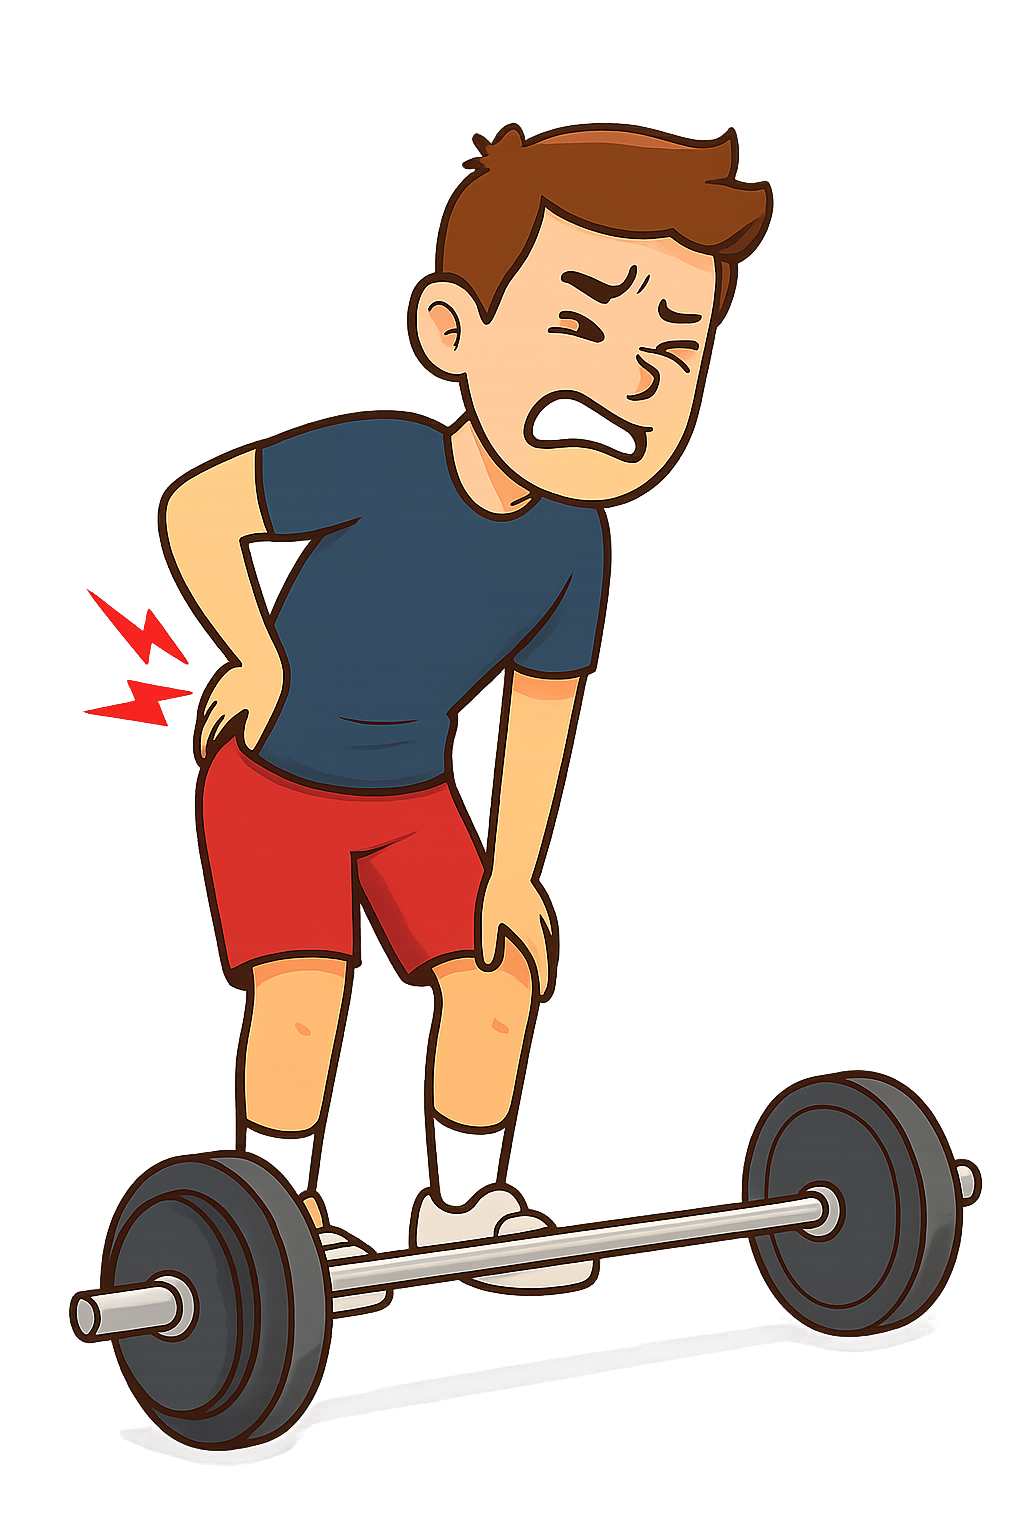
\includegraphics[width=0.45\linewidth]{cartoon_back_pain.png}
  \caption*{Foutieve uitvoering van oefening}
  \vspace{1em}
\end{figure}

Het einddoel is een gebruiksvriendelijke en technisch haalbare oplossing die nauwkeurige bewegingsanalyse mogelijk maakt. 

De proef omvat onder meer literatuuronderzoek, dataverzameling, algoritmische verwerking en evaluatie van een proof-of-concept mobiele app.

\section{Experimenten}

\begin{figure}[H]
  \centering
  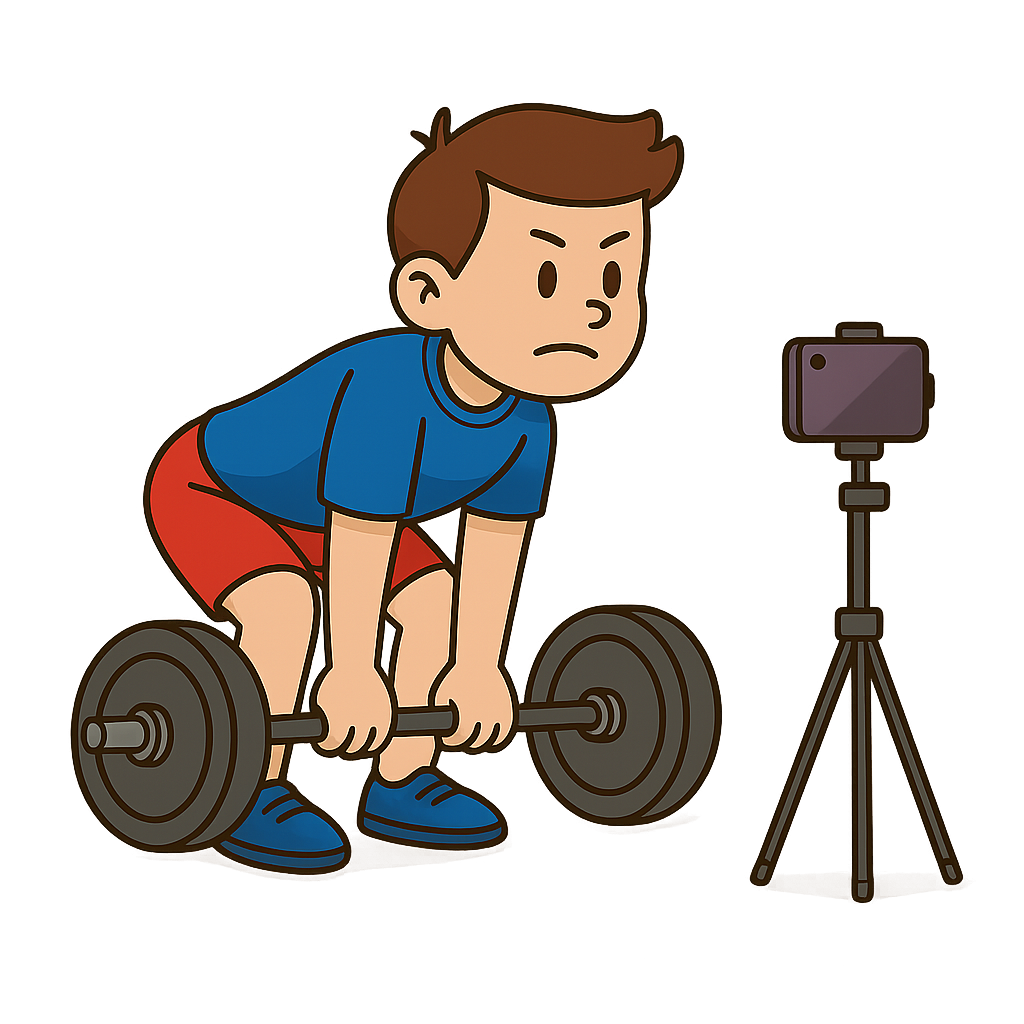
\includegraphics[width=0.45\linewidth]{cartoon_recording.png}
  \caption*{Foutieve uitvoering van oefening}
  \vspace{1em}
\end{figure}

 Voor de oefeningen squat, bench press en deadlift werden op basis van literatuurstudie biomechanische parameters vastgelegd, zoals gewrichtshoeken en bewegingspatronen, waarmee correcte en foutieve uitvoeringen onderscheiden kunnen worden. 

 De applicatie maakt gebruik van het MoveNet Lightning-model, gekozen omwille van zijn snelheid en accuraatheid, ideaal voor realtime analyse op mobiele toestellen. 

 Gebruikers uploaden een eigen video en een referentievideo; via Dynamic Time Warping worden beide uitgelijnd en frame per frame vergeleken. 

 Op basis van verschillen in vier centrale hoeken (bv. heup-knie-enkel) wordt feedback gegenereerd, visueel versterkt met kleurcodering. 

 \vspace{1em}

\begin{figure}[H]
  \centering
  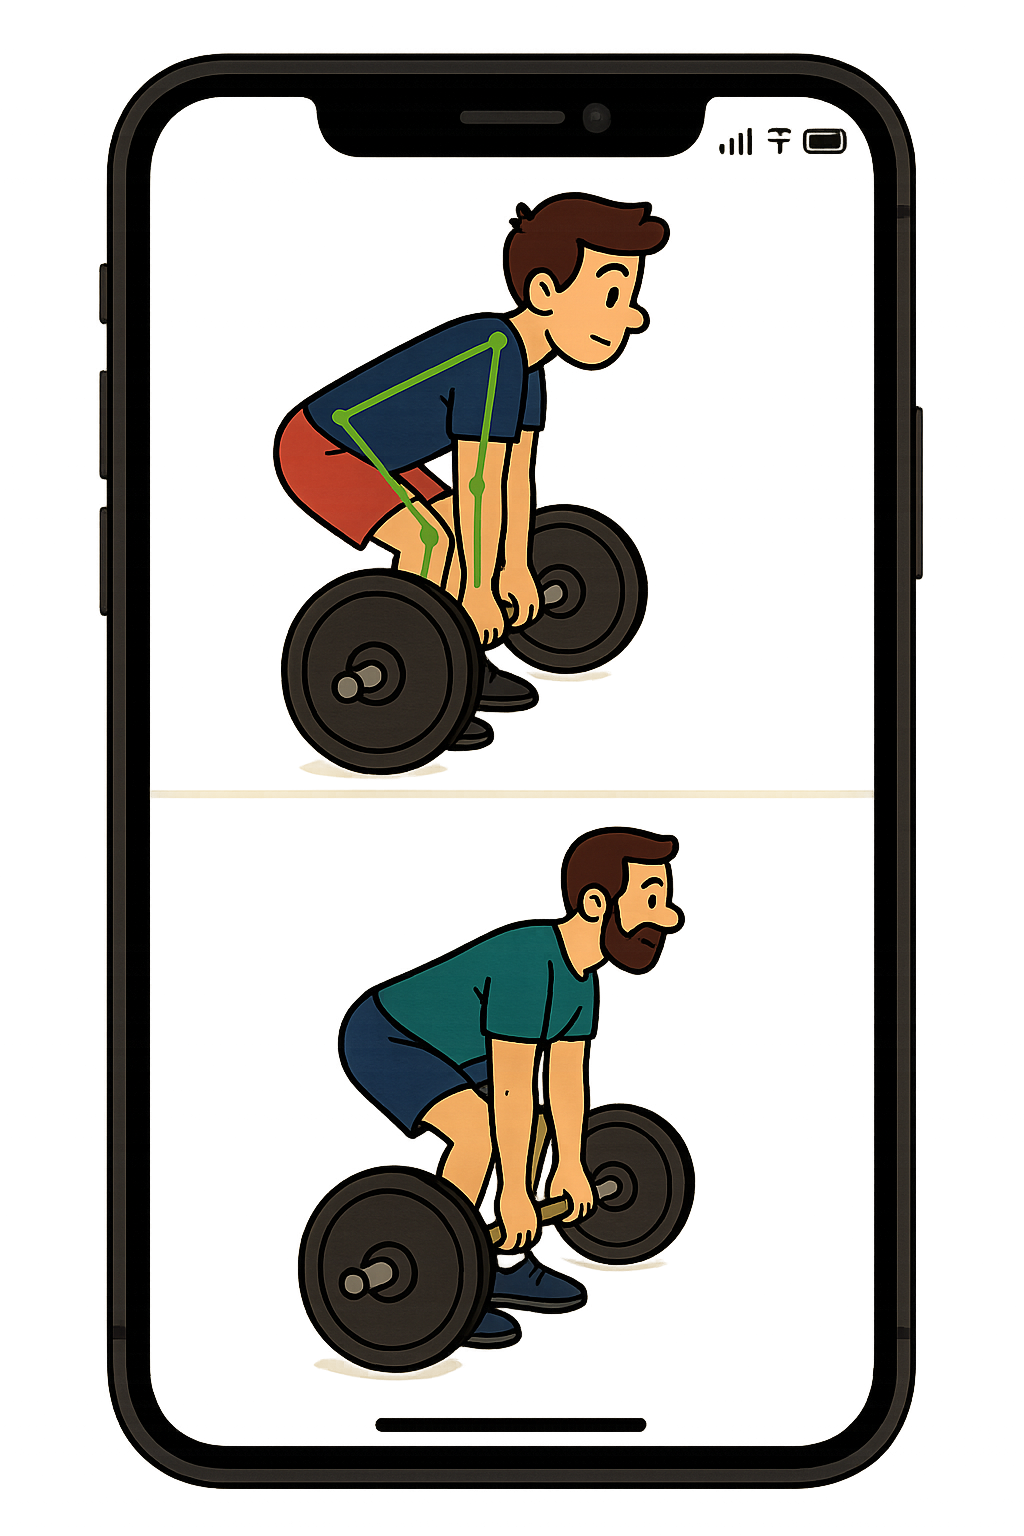
\includegraphics[width=0.45\linewidth]{cartoon_app.png}
  \caption*{Foutieve uitvoering van oefening}
  \vspace{1em}
\end{figure}

 Evaluaties tonen aan dat de applicatie betrouwbaar techniekfouten herkent, zoals een bolle rug bij de squat of een te brede grip bij de bench press. 

 Kleine meetafwijkingen door beperkingen van het algoritme blijven binnen een aanvaardbare marge. Bovendien is het systeem robuust tegen variaties in lichaamsbouw en camerahoek.

 Dit maakt het inzetbaar voor gepersonaliseerde feedback, zonder nood aan calibratie. Het eindresultaat is een flexibele, platformonafhankelijke tool voor trainers en sporters.

\section{Conclusies}

\begin{figure}[H]
  \centering
  
\includegraphics[width=0.45\linewidth]{cartoon_happy.png}
  \caption*{Foutieve uitvoering van oefening}
  \vspace{1em}
\end{figure}
 
De ontwikkelde applicatie toont aan dat het mogelijk is om krachttrainingstechniek automatisch en accuraat te analyseren via pose estimation en hoekvergelijking. 

Door gebruik te maken van MoveNet en Dynamic Time Warping wordt realtime en visuele feedback gegenereerd, wat helpt bij blessurepreventie en prestatieverbetering. 

Hoewel er nog beperkingen zijn, zoals het ontbreken van automatische correctie-adviezen en analyse vanuit meerdere hoeken, vormt dit werk een waardevolle stap in digitale trainingsondersteuning.

\section{Toekomstig onderzoek}

Toekomstig onderzoek kan zich richten op het integreren van multi-view of 3D-analyse om ook rotaties en asymmetrieën te detecteren. 

Daarnaast is het ontwikkelen van automatische foutclassificatie met concrete tekstuele feedback cruciaal om de toepasbaarheid voor eindgebruikers te vergroten. 

Tenslotte is uitgebreid gebruikersonderzoek nodig om de gebruiksvriendelijkheid en effectiviteit van de feedback in realistische sportomgevingen te valideren.

\end{multicols}
\end{document}